\section{Data Design}
\label{sec:data-design}

Data design of the solution is very simple. Table \lstinline{scanner} holds the supported scanner and its contents are constant, they do not change during runtime. Table \lstinline{report} is used to store report metadata. Tables \lstinline{vulnerability} and \lstinline{misconfiguration} store the findings extracted from the reports. Figure~\ref{img:er-diagram} depicts those entities and relationshipes between them.

\begin{figure}[!hbt]
	\begin{center}
		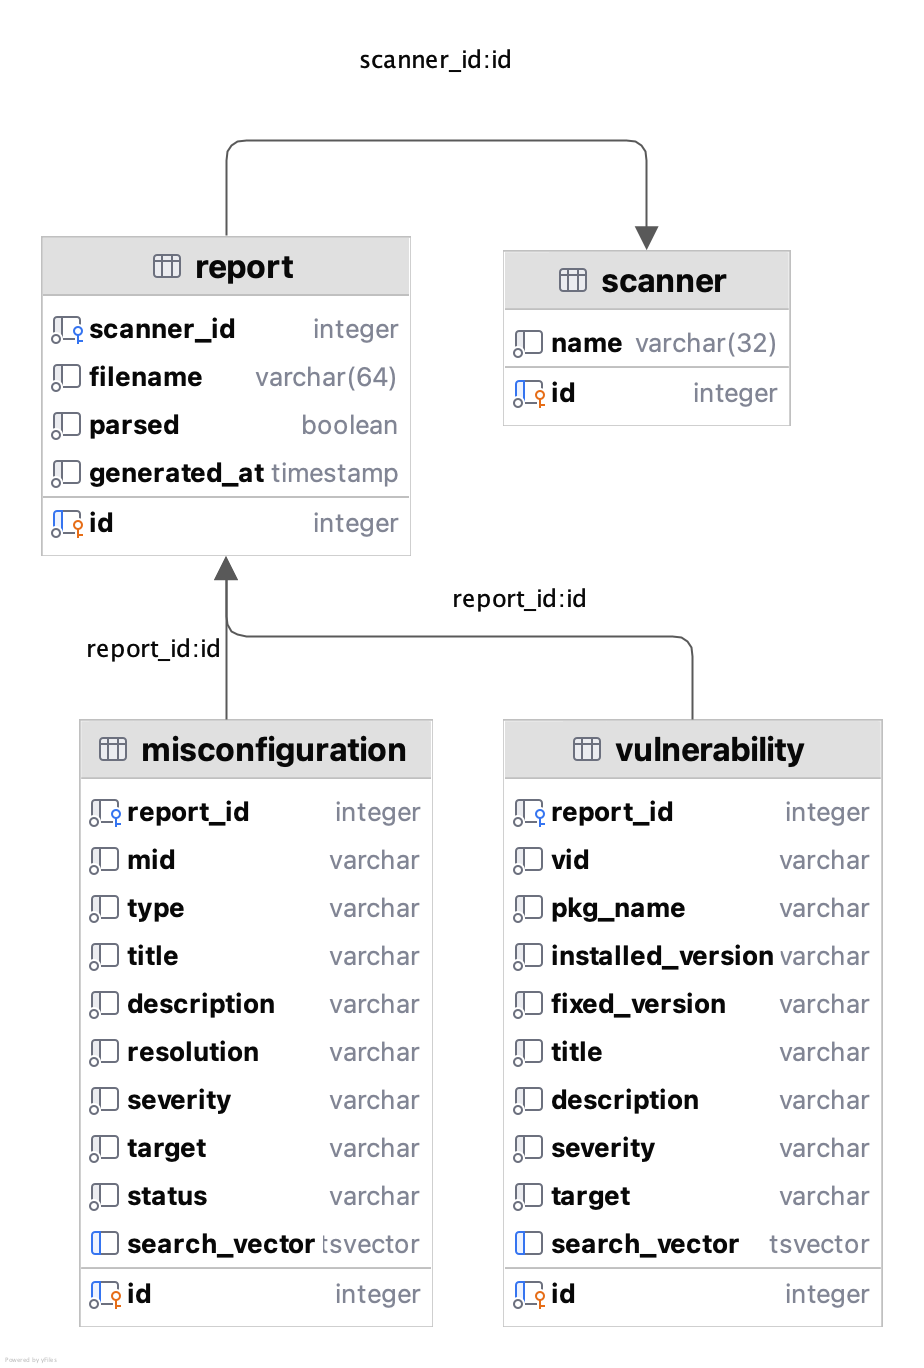
\includegraphics[width=0.5\textwidth]{images/er-diagram.png}
        \caption[Entity relationship diagram visualizing the KSA dashboard database tables and their relationship.]{Entity relationship diagram visualizing the KSA dashboard database tables and their relationship. Icons next to the column names provide necessary information about the column. Little circle in the bottom left corner depicts \lstinline{NOT NULL} constraint. Golden key denotes primary key and blue key denotes foreign key. Blue side indicates that this column is indexed.}
		\label{img:er-diagram}
	\end{center}
\end{figure}

Notice that both \textbf{vulnerability} and \textbf{misconfiguration} tables have \textbf{search\_vector} column. This column is generated when a new row is inserted or updated and used for the full-text search on these tables. Listing~\ref{lst:db-search-vector} shows the definition of the respective triggers for this column, which transform certain fields like misconfiguration id, description and title into tokens, which are then used to perform search like this: \lstinline{search_vector @@ plainto_tsquery(%s)}, where \lstinline{%s} is substitute string for the query.

\begin{lstlisting}[language=SQL, caption={[Search vector definition for misconfiguration inside the database initial script] Search vector definition for \lstinline{misconfiguration} inside the database initial script.}, label={lst:db-search-vector}]
    alter table misconfiguration 
        add column search_vector tsvector;
    create index misconfiguration_search_vector_idx on 
        misconfiguration using gin (search_vector);
    
    create function misconfiguration_update_search_vector() 
        returns trigger as $$
    begin
        new.search_vector := to_tsvector('english', new.mid ||
         ' ' || new.type || ' ' || new.title || ' ' ||
          new.description || ' ' || new.target);
        return new;
    end;
    $$ language plpgsql;
    
    create trigger misconfiguration_search_vector_trigger
    before insert or update on misconfiguration
    for each row execute function 
        misconfiguration_update_search_vector();
\end{lstlisting}